\documentclass[fleqn]{article}
\usepackage[pagebackref=false,colorlinks,linkcolor=black,citecolor=blue]{hyperref}

\usepackage[a4paper,top = 3.5 cm,bottom = 3.5 cm,left = 2 cm,right = 2cm]{geometry}
\usepackage{amsmath}
\usepackage{indentfirst}
\usepackage{mathtools}
\usepackage{amssymb}
\usepackage{amsmath}
\usepackage{amsfonts}
\usepackage{amsthm}
\usepackage{bm}
\usepackage{textcomp}
\usepackage{gensymb}
\usepackage[usenames,dvipsnames]{color,xcolor}
\definecolor{mygreen}{RGB}{28,172,0} % color values Red, Green, Blue
\definecolor{mylilas}{RGB}{170,55,241}
\usepackage{listings}
\usepackage{hyperref}
\usepackage{graphicx}
\usepackage{emptypage}
\usepackage{afterpage}
\usepackage{verbatim}
\usepackage{enumitem}
\usepackage{siunitx}
\newcommand\blankpage{%
	\null
	\thispagestyle{empty}%
	\addtocounter{page}{-1}%
	\newpage}
\usepackage{pdfpages}
\usepackage{tikz}
\usepackage[american]{circuitikz}
\usepackage{pgfplotstable}
\usepackage{pgfplots}
\usepgfplotslibrary{external} 
\tikzexternalize
\usepackage{amsthm}
\newtheorem{theorem}{قضیه}[section]
\theoremstyle{definition}
\newtheorem{definition}{تعریف}[section]

\usetikzlibrary{circuits.logic.US} % TiKZ Library for US Logic Circuits.

\usepackage{textcomp}
\usetikzlibrary{shapes,arrows,automata,positioning,calc,fit}

\usepackage{tocloft}
\usepackage{tikz}
\usetikzlibrary{positioning}
%\renewcommand{\cfttoctitlefont}{\normalfont\Large}% Remove \bfseries from ToC title
\renewcommand{\cftsecfont}{}% Remove \bfseries from section titles in ToC
\renewcommand{\cftsecpagefont}{}% Remove \bfseries from section titles' page in ToC
\usepackage[american]{circuitikz}
\usetikzlibrary{calc}
\usetikzlibrary{decorations.markings}
\usepackage{xepersian}
\settextfont{XB Niloofar}
\makeatletter
\makeatother
\renewcommand{\baselinestretch}{1}

\begin{document}

\begin{titlepage}
    \centering
    \settextfont{Amiri}
    \huge
    باسمه تعالی
    \\
    \vspace{0.5 cm}
    \settextfont{XB Niloofar}
    \begin{figure}[h!]
        
\includegraphics[width=4 cm]{logo.png}
        \centering
    \end{figure}
    \huge
    \textbf{دانشگاه صنعتی شریف}
    \vspace{1.5 cm}
    \Huge

    \textbf{پروژه درس سیگنال ها و سیستم ها}
    \huge

    \vspace{1.2 cm}
    % حذف نویز برق شهری با فیلتر های وفقی
    % \vspace{l}
    دانشکده مهندسی برق

    \vspace{0.5 cm}
    نیم سال دوم ۱۴۰۱-۱۴۰۲

    \vspace{1.5 cm}
    امیررضا ولائی \quad 400102222\\
    احسان مریخی \quad 400101967

\end{titlepage}
\large
\noindent

\section{سیگنال های تک تن و سیگنال های ویژه ها}

برای سیگنال های تک تن پیوسته داریم:
$$x(t)=Ae^{j(\omega t + \phi)}$$
اگر فرض کنیم پاسخ ضربه سیستم $h(t)$ باشد، داریم:
\begin{gather*}
    y(t)=x(t)*h(t)\rightarrow y(t)=\sum_{\theta=-\infty}^{\infty}Ae^{j(\omega(t-\theta) + \phi)}h(\theta)=Ae^{j(\omega t + \phi)}\sum_{\theta=-\infty}^{\infty}Ae^{-j\omega \theta}h(\theta) \\
    y(t)=\lambda x(t)
\end{gather*}
برای سیگنال های تک تن گسسته داریم:
\begin{gather*}
    x[n]=Ae^{j(\omega n + \phi)}
\end{gather*}
اگر فرض کنیم پاسخ ضربه سیستم $h[n]$ باشد و $x[n]$ متناوب باشد، آنگاه
\begin{gather*}
    y[n]=x[n]*h[n]\rightarrow y[n]=\sum_{\theta=-\infty}^{\infty}Ae^{j(\omega(n-\theta) + \phi)}h[\theta]=Ae^{j(\omega n + \phi)}\sum_{\theta=-\infty}^{\infty}Ae^{-j\omega \theta}h[\theta] \\
    y[n]=\lambda x[n]
\end{gather*}

بنابراین نتیجه میگیریم به صورت کلی سیگنال های تک تن سیگنال ویژه های سیستم هستند؛ به صورتی که اگر وارد سیستم شوند، خروجی ضریبی از ورودی خواهد بود.

\section{ویژگی سیگنال های ویژه}
می دانیم که $e^{j\omega}$ ها سیگنال ویژه های یک سیستم LTI هستند. می توانیم $\cos(2\pi 50 n)$ و $\sin(2\pi 50 n)$ را به صورت زیر بنویسیم:
\begin{gather*}
    \cos(2\pi 50 n)=\frac{e^{j2\pi 50 n}+e^{-j2\pi 50 n}}{2} \\
    \sin(2\pi 50 n)=\frac{e^{j2\pi 50 n}-e^{-j2\pi 50 n}}{2j}
\end{gather*}
در نتیجه می توانیم بگوییم که $\cos(2\pi 50 n)$ و $\sin(2\pi 50 n)$ نیز سیگنال های ویژه هستند و اگر ورودی ترکیب خطی از آن ها باشد، بنا به اصل \textit{\lr{Super position}} خروجی نیز ترکیب خطی از خروجی های آن ها خواهد بود و تنها با دو ضریب می‌توانیم خروجی را با استفاده از پایه های $\sin(2\pi 50 n)$ و $\cos(2\pi 50 n)$ بنویسیم.\\





\section{\lr{Gradient Descent}}
الگوریتم (GD) یا \lr{Gradient descent} یکی از الگوریتم های مهم در مسئله یافتن پاسخ بهینه سازی برای توابع Convex هست. هرچند تعمیم هایی از این الگوریتم برای توابع غیر محدب نیز استفاده می‌شود که در آن مسائل بجای یک پاسخ بهینه برای هر نقطه شروع، ممکن است به نقاط بهینه مختلفی دست پیدا کنیم.\\
یک تابع در صورتی محدب یا Convex می‌باشد که رابطه ریاضی زیر برقرار باشد:\\
\begin{gather*}
    f(\alpha x + (1-\alpha)y) \leq \alpha f(x) + (1-\alpha)f(y) \quad \forall x,y \in \mathbb{R}^n, \alpha \in [0,1]
\end{gather*}
یا به زبان ساده، اگر برای هر دو نقطه $x,y$ در تابع $f$، نقطه میانی $z$ وجود داشته باشد که مقدار تابع در آن نقطه کمتر از میانگین مقدار تابع در $x,y$ باشد، آنگاه تابع $f$ محدب است.\\
\begin{figure}[h!]
    \centering
    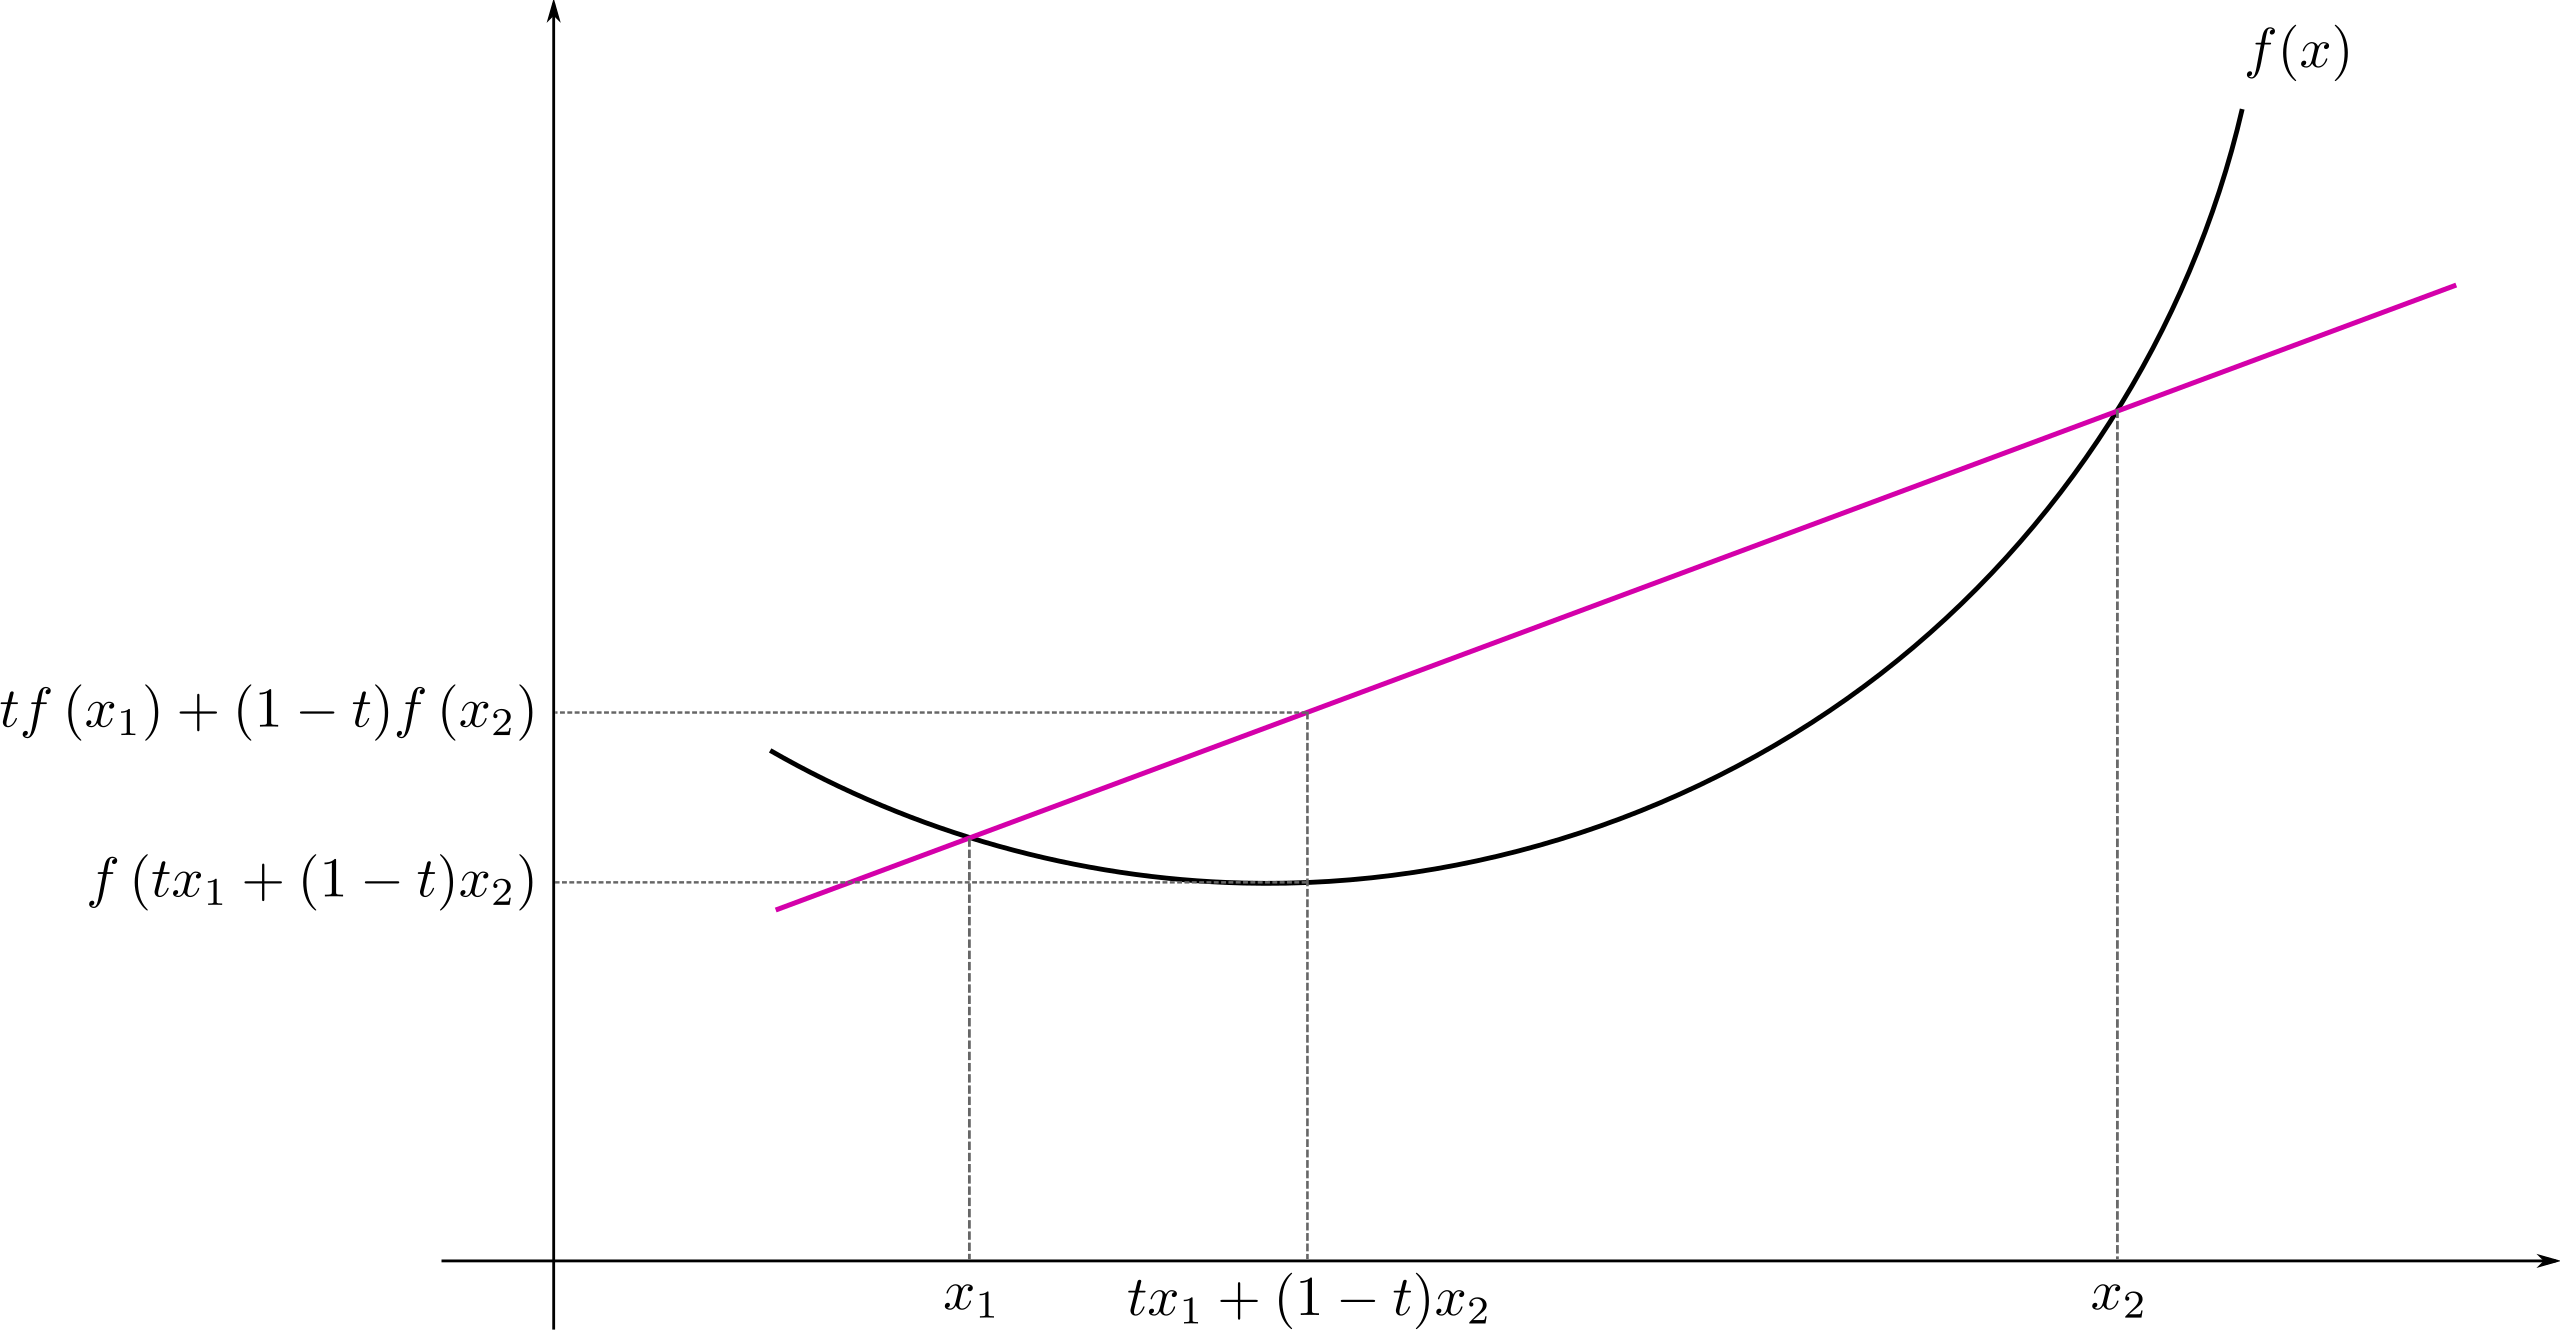
\includegraphics[width=0.6\linewidth]{./Pics/ConvexFunction.png}
    \caption{تابع محدب}
    \label{fig:convex}
\end{figure}
\\
می‌دانیم که گرادیان یک تابع در هر نقطه، جهت بیشینه را نشان می‌دهد. بنابراین اگر در هر نقطه، به جای حرکت در جهت گرادیان، در جهت عکس گرادیان حرکت کنیم، مقدار تابع کمتر می‌شود. این روش به روش کاهش گرادیان یا \lr{Gradient Descent} معروف است.\\
\\
\subsection{ﺍﺛﺒﺎﺕ ﺍﻓﺰﺍﯾﺶ ﻣﻘﺪﺍﺭ ﺗﺎﺑﻊ ﺩﺭ ﺟﻬﺖ گرﺍﺩﯾﺎﻥ}
اگر تابع چند متغیره $f(x_1,x_2,...,x_n)$ را در نظر بگیریم، گرادیان آن به صورت زیر تعریف می‌شود:\\
\begin{gather*}
    \nabla f = \left[\frac{\partial f}{\partial x_1},\frac{\partial f}{\partial x_2},...,\frac{\partial f}{\partial x_n}\right]^T
\end{gather*}
که در آن: \\
\begin{gather*}
    \frac{\partial f}{\partial x_i} = \lim_{h \to 0} \frac{f(x_1,x_2,...,x_i+h,...,x_n) - f(x_1,x_2,...,x_i,...,x_n)}{h}
\end{gather*}
آنگاه برای تغییرات کوچک در $x$، تغییرات متناظر در $f$ به صورت زیر است:\\
\begin{gather*}
    f(x + \delta x) \approx f(x) + \nabla f^T \delta x = f(x) + \left\langle \nabla f, \delta x \right\rangle = f(x) + \left\| \nabla f \right\| \left\| \delta x \right\| \cos \theta
\end{gather*}
حال اگر $f(x)$ را به سمت چپ معادله ببریم، داریم:
\begin{gather*}
    f(x + \delta x) - f(x) \approx \left\| \nabla f \right\| \left\| \delta x \right\| \cos \theta
\end{gather*}
میدانیم نرم 1 یا اندازه هر بردار مقداری ثابت و مثبت است.  پس برای مثبت بودن مقدار تغییرات، باید در جهتی حرکت کنیم که $\cos \theta$ مثبت باشد، یا به عبارتی $\theta < \pi$ باشد. برای منفی بودن مقدار تغییرات نیز باید در جهتی حرکت کنیم که $\theta$ یا همان زاویه بین $\left\| \delta x \right\|$ و $\left\| \nabla f(x) \right\|$ بزرگ تر از $\pi$ باشد.\\
بیشینه تغییرات منفی زمانی رخ می‌دهد که $\cos \theta$ کمینه باشد یا به عبارتی $\theta = \pi$ باشد یا جهت تغییرات $x$ در خلاف جهت $\left\| \nabla f(x) \right\|$ باشد.
\subsection{الگوریتم Descent Gradient }
این الگوریتم برای پیدا کردن نقطه مینیمم توابع محدب (یا نقطه ماکسیسمم توابع مقعر با یکسری تغییر) استفاده میشود. صورت کلی الگوریتم به این شکل است که در هر \lr{Itratation}، در سمت عکس گرادیان حرکت میکنیم. از قسمت قبل می‌دانیم که اگر در جهت عکس گرادیان تابع محدب حرکت کنیم، مقدار خروجی تابع کمتر می‌شود؛ لذا اگر الگوریتم را به تعداد کافی \lr{iteration} با ضریب مناسب پشت گرادایان انجام دهیم؛ قطعا (مجدداً تاکید میشود که تابع باید Convex باشد یا به عبارتی ماتریس هسین تابع PD باشد) به نقطه مینیمم تابع خواهیم رسید.\\
همگرایی در این الگوریتم یا با تعداد \lr{iteration} و یا با مقدار تفاوت تابع در دو ایتریشن آخر و مقدار $\epsilon$ که در اول اجرای الگوریتم تعیین می‌شود کنترل می‌شود و در صورت ارضای هر کدام از شرط ها اجرای آن به اتمام می‌رسد.\\
برای ضریب پشت گرادیان از تعاریف مختلفی استفاده می‌شود. ساده ترین تعریف استفاده از ضریب ثابت $\eta$ پشت گرادیان است. یکی از تعاریف دیگر، استفاده از مومنتوم است:
\begin{gather*}
    m_t = \beta m_{t-1} + g_{t-1} \\
    \theta_t = \theta_{t-1} + \eta_t g_{t}
\end{gather*}
یکی از نکات مهم درمورد $\eta$ این است که اگر $\eta$ بزرگی را برای شروع انتخاب کنیم، ممکن است الگوریتم در مرز نزدیک نقطه مینیمم هیچوقت به نقطه مینیمم نزدیک نشود و تغییرات تابع در آن نقطه بسیار زیاد باشد. بالعکس، اگر مقدار $\eta$ کوچک انتخاب شود، ممکن است لازم باشد \lr{iteration} های زیادی انجام شود تا الگوریتم به نقطه مینیمم نزدیک شود.\\

\subsection{الگوریتم \lr{stochastic gradient descent}}
در این الگوریتم، در هر \lr{iteration}، یک نمونه از داده ها را انتخاب می‌کنیم و برای آن نمونه، گرادیان را محاسبه می‌کنیم و در جهت عکس آن حرکت می‌کنیم. این الگوریتم برای مسائلی که داده ها بسیار زیاد هستند و یا محاسبه گرادیان برای تمام داده ها بسیار زمان بر است، استفاده می‌شود.\\
همچنین می‌توانیم به جای انتخاب تمام \lr{data set}، بخش کوچکی از آن را انتخاب کنیم که به این الگوریتم نیز


\clearpage
\section{بلوک دیاگرام فیلتر وقفی برای فیلتر نویز برق شهری}
بلوک دیاگرام فیلترهای وفقی با کاربرد حذف نویز به صورت کلی به شکل  زیر است:
\begin{figure}[h!]
    \centering
    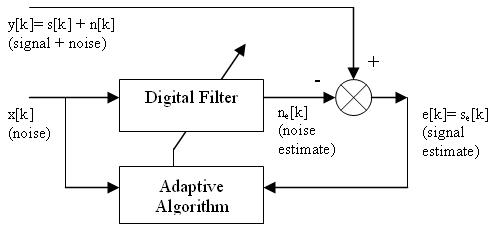
\includegraphics[width=0.6\linewidth]{./Pics/Block_diagram.png}
    \caption{بلوک دیاگرام فیلتر وفقی برای حذف نویز}
    \label{fig:BD_Adaptive Filter Noise Canseling}
\end{figure}
\\
که مشابه همان سیستمی است که در جزوه درس استاد بابائی آورده شده است:
\begin{figure}[h!]
    \centering
    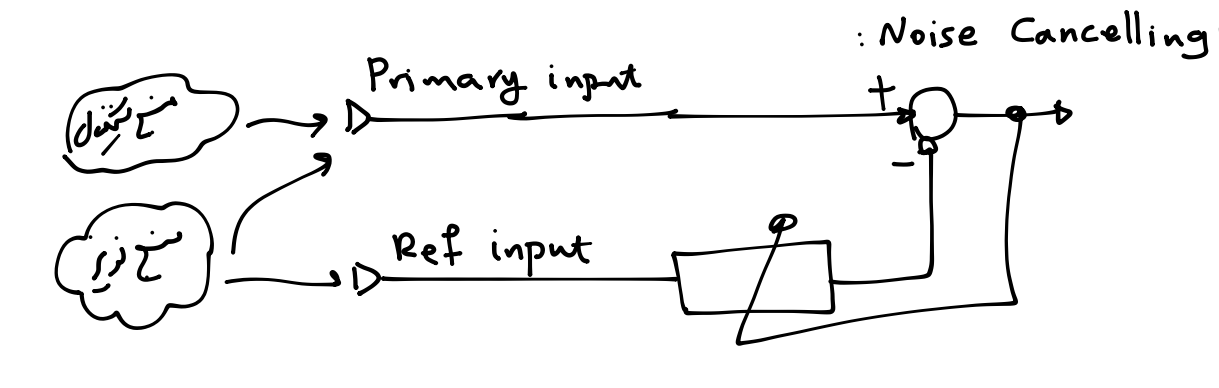
\includegraphics[width=0.4\linewidth]{./Pics/Block_diagram_BABA.png}
    \caption{فیلتر وفقی با هدف حذف نویز}
    \label{fig:BD_Adaptive Filter}
\end{figure}
\\
% Block Diagram fo Adaptive Filter for Noise Canseling
اگر بخواهیم با مشخص کردن بلوک \lr{Adaptive Algorithm} به صورت واضح تر بلوک دیاگرام فیلتر وفقی حذف نویز را نشان دهیم، داریم:
\begin{figure}
    \centering
    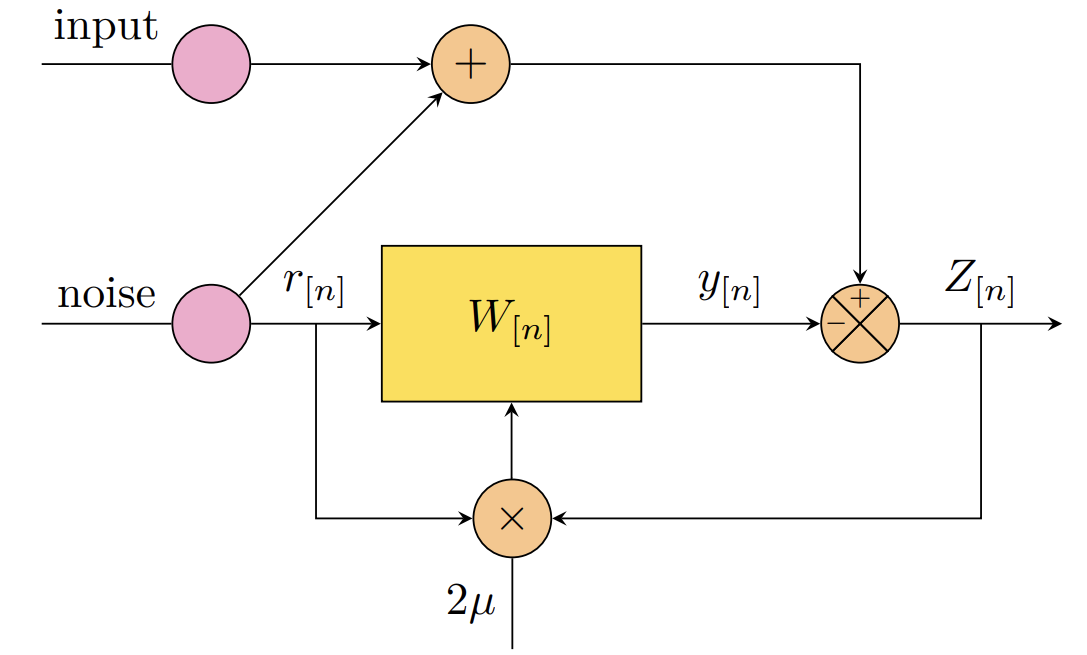
\includegraphics[width=0.5\linewidth]{./Pics/BD.png}
    \caption{فیلتر وفقی با هدف حذف نویز}
    \label{fig:BD}
\end{figure}
\clearpage



\section{مقدار $\mathbb{E}(e(n))$}
    مقدار $\mathbb{E}(e(n))$ با توجه به بلوک دیاگرام موجود برابر سیگنال ورودی بدون نویز است. یعنی:
    \begin{gather*}
        \mathbb{E}(e(n)) = \mathbb{E}(d(n) - y(n)) = \mathbb{E}(d(n)) - \mathbb{E}(y(n))
    \end{gather*}
    به عبارتی، انتظار داریم در صورت همگرایی الگوریتم $GD$، سیگنال $\mathbb{E}(e(n))$ به سیگنال ورودی بدون محتوی نویز هم‌گرا شود.\\
    به عبارتی، تنها در صورتی که سیگنال اولیه صرفا شامل نویز باشد انتظار داریم که مقدار $\mathbb{E}(e(n))$ صفر باشد (که تا حدی غیرمنطقی نیز هست).
    

    \section{حذف نویز سینوسی $50$ هرتز از وویس ریکورد شده با روش LMS }
    توضیح کلی الگوریتم پیاده سازی شده :
    در اینجا به جای استفاده از اختلاف سیگنال بدون نویز و سیگنال تخمین به عنوان تابع خطا از خود سیگنال تخمین به عنوان خطا استفاده میکنیم.
    هدف مینیمم کردن این تابع خطا می‌باشد که از الگوریتم LMS کمک میگیریم تا به این هدف برسیم.
    در این الگوریتم یه تابع وزن داریم که در هر مرحله نویز رفرنس را آپدیت میکند تا شبیه به نویز روی سیگنال اصلی شود.
    در هر مرحله تابع وزن خودش را با کمک تابع خطا آپدیت میکند تا به حالت اپتیمال برسد.
    \\
    تاثیر مقدار $\mu$ روی همگرایی و دقت :
    با انتخاب بزرگتر مقدار $\mu$ سرعت همگرایی بیشتر میشود اما دقت آن کمتر میشود.
    دلیل این اتفاق این است که تابع وزن سریعتر میتواند به مقدار اپتیمال نزدیک شود اما وقتی به آن نزدیک میشود به خاطر بزرگ بودن $\mu$ نمیتواند خود را به اپتیمال ترین حالت ممکن برساند.
    همچنین اگر $\mu$ بسیار کوچک انتخاب شود دفت همگرایی زیاد میشود اما سرعت همگرایی کم میشود.
    \clearpage
    در این بخش از کد با ران گرفتن می‌توانیم 5 ثانیه وویس گرفته و آن را با نام audio.wav سیو کنیم.
    \begin{figure}[h!]
        \centering
        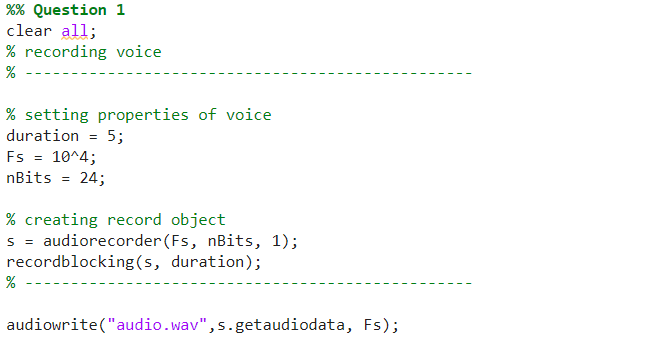
\includegraphics[width=0.4\linewidth]{Pics/Screenshot (181).png}
        \caption{ایجاد و ذخیره فایل صدا}
        \label{fig:Saving voice}
    \end{figure}
    \\
    با ران کردن این بخش ابتدا فایل با نام audio.wav خوانده میشود و سپس سیگنال سینوسی 50 هرتز با فاز اولیه رندوم و مقدار $0.5$ به آن اضافه میشود.
\begin{figure}[h!]
    \centering
    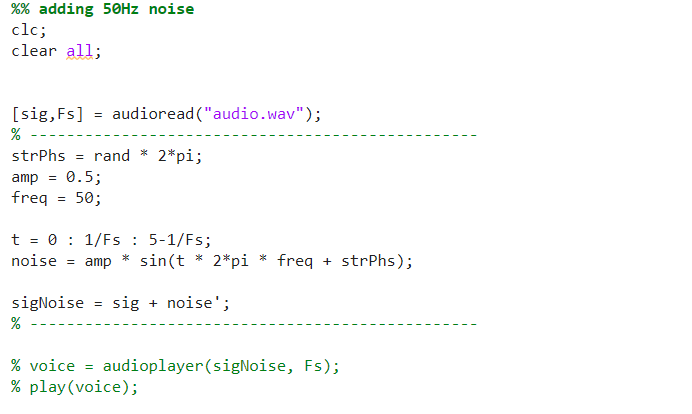
\includegraphics[width=0.4\linewidth]{Pics/Screenshot (182).png}
    \caption{اضافه کردن نویز به فایل صدا}
    \label{fig:Adding noise}
\end{figure}
\\
در این بخش ابتدا نویز با جنس یکسان اولیه اما با فاز متفاوت از آن ایجاد میکنیم. سپس از آن به عنوان نویز رفرنس در الگوریتم LMS استفاده میکنیم.
\begin{figure}[h!]
    \centering
    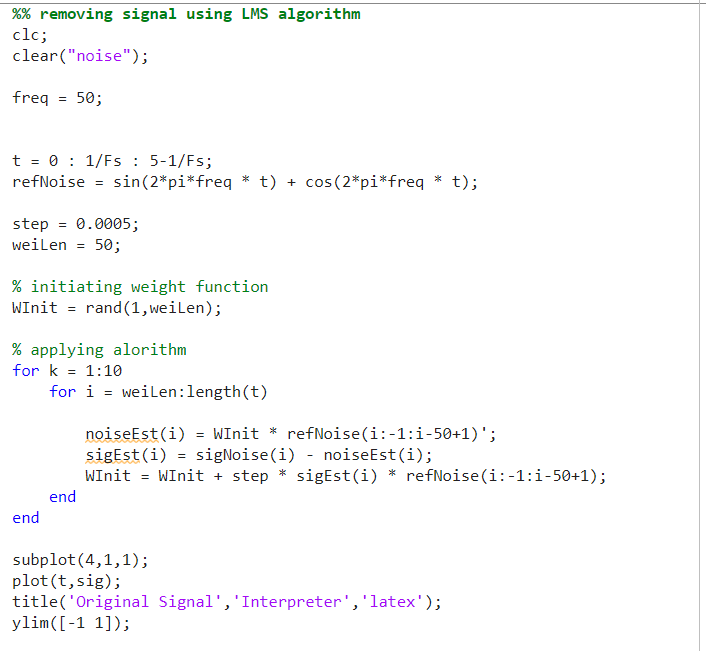
\includegraphics[width=0.4\linewidth]{Pics/Screenshot (183).png}
    \caption{حذف کردن نویز با الگوریتم LMS}
    \label{fig:Removing noise}
\end{figure}


\newpage
\clearpage
\section{حذف نویز سینوسی $50$ هرتز از وویس ریکورد شده با روش LMS}
ابتدا فایل دیتای داده شده رو لود کرده و فرکانس سمپلینگ و محتوی آن را جدا میکنیم.
\begin{figure}[h!]
    \centering
    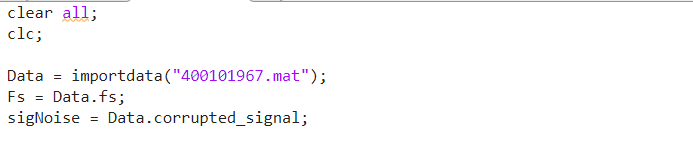
\includegraphics[width=0.4\linewidth]{Pics/Screenshot (184).png}
    \caption{خواندن دیتا}
    \label{fig:Read data}
\end{figure}
\\
سپس کاملا مشابه با سوال قبل همان الگوریتم را پیاده سازی کرده و با استفاده از نویز رفرنس نویز موجود در دیتا را حذف میکنیم.
\begin{figure}[h!]
    \centering
    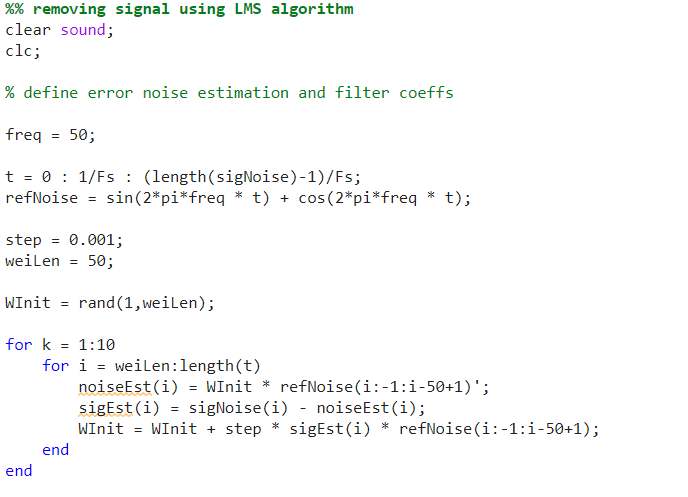
\includegraphics[width=0.4\linewidth]{Pics/Screenshot (185).png}
    \caption{حذف نویز از دیتا}
    \label{fig:Remove Noise}
\end{figure}


\end{document}
